\documentclass{article}
\usepackage{graphicx}
\usepackage[margin=1in]{geometry}

\begin{document}
\begin{titlepage}
	\clearpage\thispagestyle{empty}
	\centering
	\vspace{1cm}
		
	\rule{\linewidth}{1mm} \\[0.5cm]
	{ \Large \bfseries ISyE 6740 - Spring 2021\\[0.2cm]
		Final Report}\\[0.5cm]
	\rule{\linewidth}{1mm} \\[1cm]
	
		\begin{tabular}{l p{5cm}}
		\textbf{Team Member Names:} &  Koh Rui Nah \\[10pt]
		\textbf{Project Title:} & Finding the hottest topics in Tech \\[10pt]
		\textbf{Please include (at least) the following sections.} & \\
		\end{tabular} 

        \begin{itemize}
            \item[] \textbf{Problem Statement}
            
           \quad  Technology (Tech) is a domain in a constant flux. New technology and terms have emerged rapidly over time. As a result, people and by extension organizations, find it hard to keep track of these trends and are often lost in a sea of topics. For example, we know that artificial intelligence (ai) is a hot topic in the recent years. However, we are unable to tell its various applications in other domains.
           
            \quad This project aims to use natural language processing techniques to analyse tech articles from online sources, derive topics from these articles, and analyse tech trends to allow easier monitoring of such trends across a period of time. There have been studies and projects to classify news articles into their different topics using the BBC news dataset. However these are based on broad topics (business, entertainment, politics, sport or tech.) which do not drill down into the different subtopics of each domain. This project would allow tech professionals and corporate communications teams to better understand the landscape and quickly detect emerging trends within a tech domain.
            
            \item[] \textbf{Data Source}
            
            \quad The data source consisted of tech articles from tech websites such as techradar, wired etc.and mainstream news sites focused on reporting tech news such as reuters, new york times and the guardian etc. Data was retrieved by querying the newsapi with keywords related to the categories of interest namely: ai, cybersecurity, electric vehicles, cloud (computing), blockchain and digitalisation. These keywords acted as a label for validation purposes. The api returned links  and information to the articles including a short summary. As the short summary is insufficient to do textual analysis, we used newspaper3k to obtain the full article using the link provided by the api. The dataset includes the columns date, title, source, blurp, text and label. 
            
            \quad For the training set, a total of 1200 articles were retrieved and after preprocessing, a step which will be explained later, there were 480 articles remaining with a vocabulary size of 74556. As newsapi only allows users to query articles from a month ago, the dates of the articles ranged from 25 Mar 2022 to 22 Apr 2022. 
             
             \quad  The test set consisted of 71 articles from 22 Apr 2022 to 27 Apr 2022. This was to mimic a real use case where a company uses the model on a new and recent set of data. 
           
\begin{center}
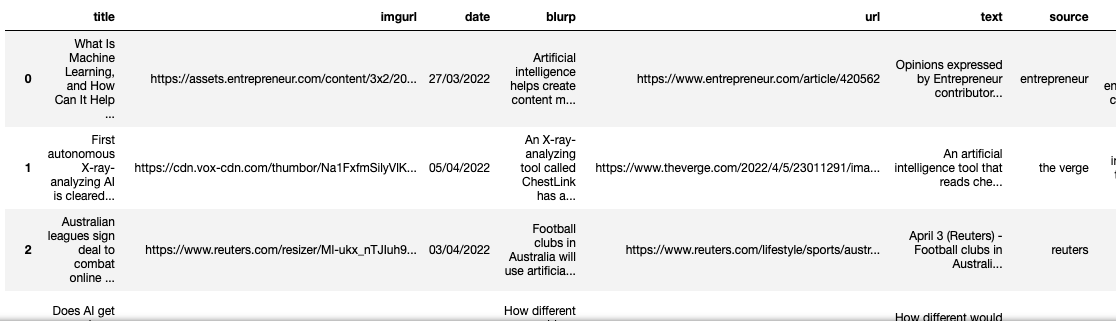
\includegraphics[width = 0.9\textwidth]{datasource}
\end{center}           
           
            
            \item[] \textbf{Methodology}
          	
          	\quad This section will cover the methodology used in the preprocessing for the text column. This included: the removal of duplicates from the articles, the grouping of articles with multiple categories together (ie. an article can be both about blockchain and artificial intelligence), the elimination of short articles with less than  the removal of punctuation, numbers, and stopwords, using pos tagging using the spacy package to remove intermediate words such as prepositions, adverbs verbs, modal verbs (to ensure that the model is able to pick up the correct keywords), tokenization of the text to form individual words as well as the creation of a bigram model to ensure words such as artificial intelligence will be considered as a single entity compared to separate words.
          	
			\quad To ensure words with the same base to be recognized as a single entity, lemmatization was performed. Lemmatization considers the context of the word before converting it to its base form (eg. data to datum, vehicles to vehicle). 
            
             \quad The data from the text column was transformed into a document term matrix. Each row of the data would be an article (document), while the features will be the words from the article (Each column represents a word). This forms the corpus to perform topic modelling on.
            
            \quad Topic modelling using latent dirichlet allocation (LDA) (Blei et al., 2003) was used to obtain topics from these articles. The assumptions following LDA are that 1) articles (or documents) contain different topics 2) topics are formed by a mixture of words. As such, words are being generated by a probability distribution of each topic, while articles form the probability distribution of topics. The number of documents will be represented by the variable M, whereas the number of words will be N.
            
           	\quad LDA breaks down the document (article) word matrix into two separate matrices, the document topic matrix and the topic word matrix. The former matrix will have a chosen number of topics which form the columns, while the documents form the rows. For the latter, the rows are denoted by topics and the columns will be the words a topic contains.
            
            \quad Following LDA approach, each word will have a latent (related) topic represented by Z. The probability of Z being assigned to a topic will follow $\theta$ which is the topic distribution. LDA possesses two controls: $\alpha$ and $\beta$. $\alpha$ controls the document topics distribution, whereas $\beta$ controls for the topic word distribution. A higher $\alpha$ would result in documents having more topics while lower $\alpha$ results in less. For $\beta$ the higher it is the more words appear in a given topic and vice versa. This project utilized the gensim package with alpha set as 'auto' allowing the algorithm to learn the prior asymmetric prior from the corpus. Similarly beta or 'eta' in gensim, was set to auto to learn the asymmetric prior. Attempting to change either alpha or beta into symmetric or asymmetric resulted in less coherent topics and a larger divergence from the original keyword which was queried.
            
      		\quad According to Gan and Qi, the LDA algorithm ranks words based on the probability distribution and use this result as their output. This ranking of words in turn represents the importance of the word to the topic. The results returned by the algorithm will be in the form of words and the given weights for the topics ie. which words represent a given topic:
	
\begin{center}
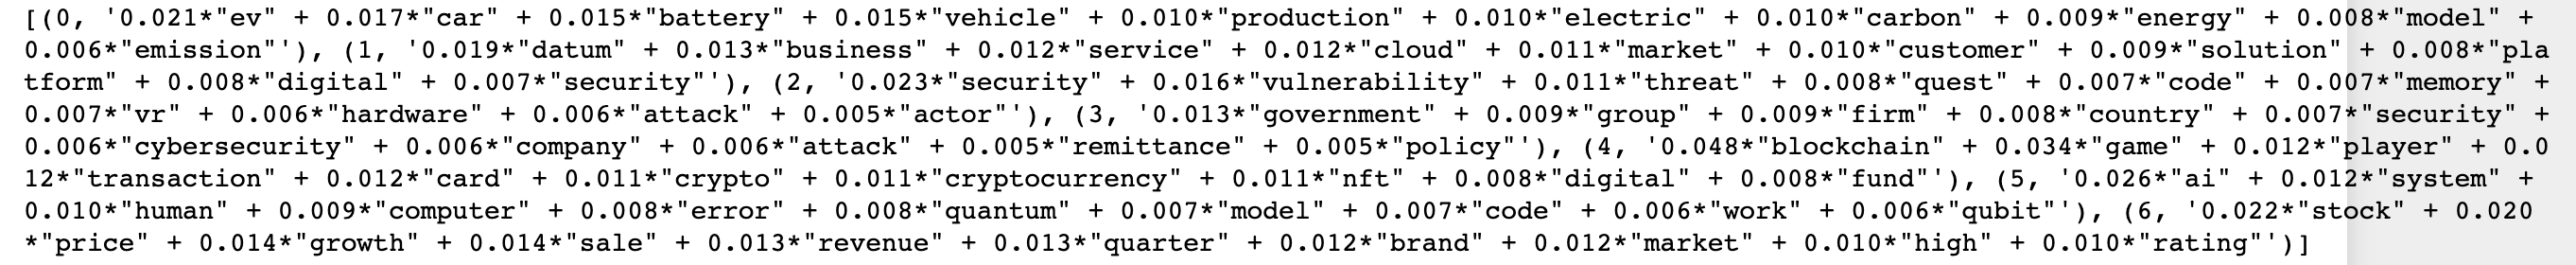
\includegraphics[width = 0.9\textwidth]{weighted_tokens}
\end{center}
 
 
 			\quad To determine the optimal number of topics for the LDA model, we took a two pronged approach. First, this study trialled a varying number of topics for LDA before settling on be 7 topics after analysing the keywords tagged to each topic and the plot by PyLDAvis to ensure that the topics had a good intertopic distance. Second, the number of topics was decided by selecting the model with the highest coherence score. 
 			
 				
			\quad Once the model was trained with the determined number of topics, we obtain the topic distribution for each document and assign the topic to the document if the probability is above the threshold of 0.2. 
 			
 \begin{center}
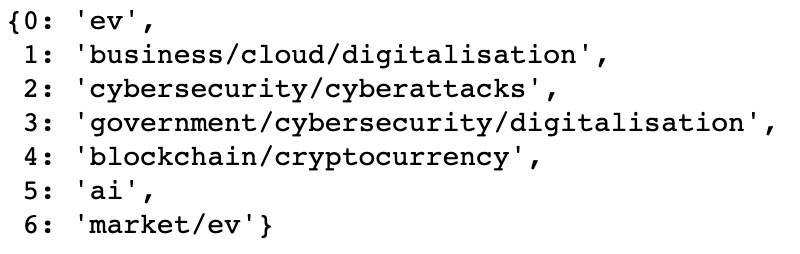
\includegraphics[width = 0.7\textwidth]{topic_dict}
\end{center}
 			
 			
 			
			\quad Taking into account the words and weights from the given output, human intuition was required to determine a logical "topic" from the weighted tokens. This requires an understanding of the topic covered (for example a combination of ev, energy, vehicle and car could be referring to the topic on Electric Vehicles).  This step relied on human judgement as it requires a human to decide the overall topic. Unlike the keyword (categories) which were used to query the api (artificial intelligence, digitalisation etc.), the topics tended to be broader than these categories and usually included a mix of categories. This means some other contextual categories were added for informational purposes. For example, cybersecurity was linked to government, while digitalisation also appeared frequently with cloud. Increasing the number of topics did not result in the segregation of topics. This could mean that the topics selected beforehand were subtopics of a larger topic. As such, the topics assigned to the articles by LDA had multiple categories. Hence, several categories from the original queries had to be merged together. 
			
			\quad To ensure that the merging was systematic, the rule applied was as such: if the category of interest (among the 6 original queried keywords) or its synonym appears in the top 30 (usually top 10) it can be included in the current topic. Topic 0 is largely about electric vehicles and the companies selling them. Topic 2 covers cloud platforms and services as well as how business utilize them for digital transformation. Topic 3 is related to cybersecurity issues, ranging from cyber attacks to threats and vulnerabilities, and security issues as well. Topic 4 covers blockchain and crypotocurrency, covering subjects such as bitcoin, ethereum and nfts. Topic 5 encompasses artificial intelligence and its use cases. Topic 6 covers market related issues. This consisted of stock prices, sales, growth, profits, revenue of companies. The category of Electric vehicles was included as it is a hot subject within this topic.
            
		
			
            \pagebreak
            
            \item[] \textbf{Evaluation and Final Results}
            
\begin{center}
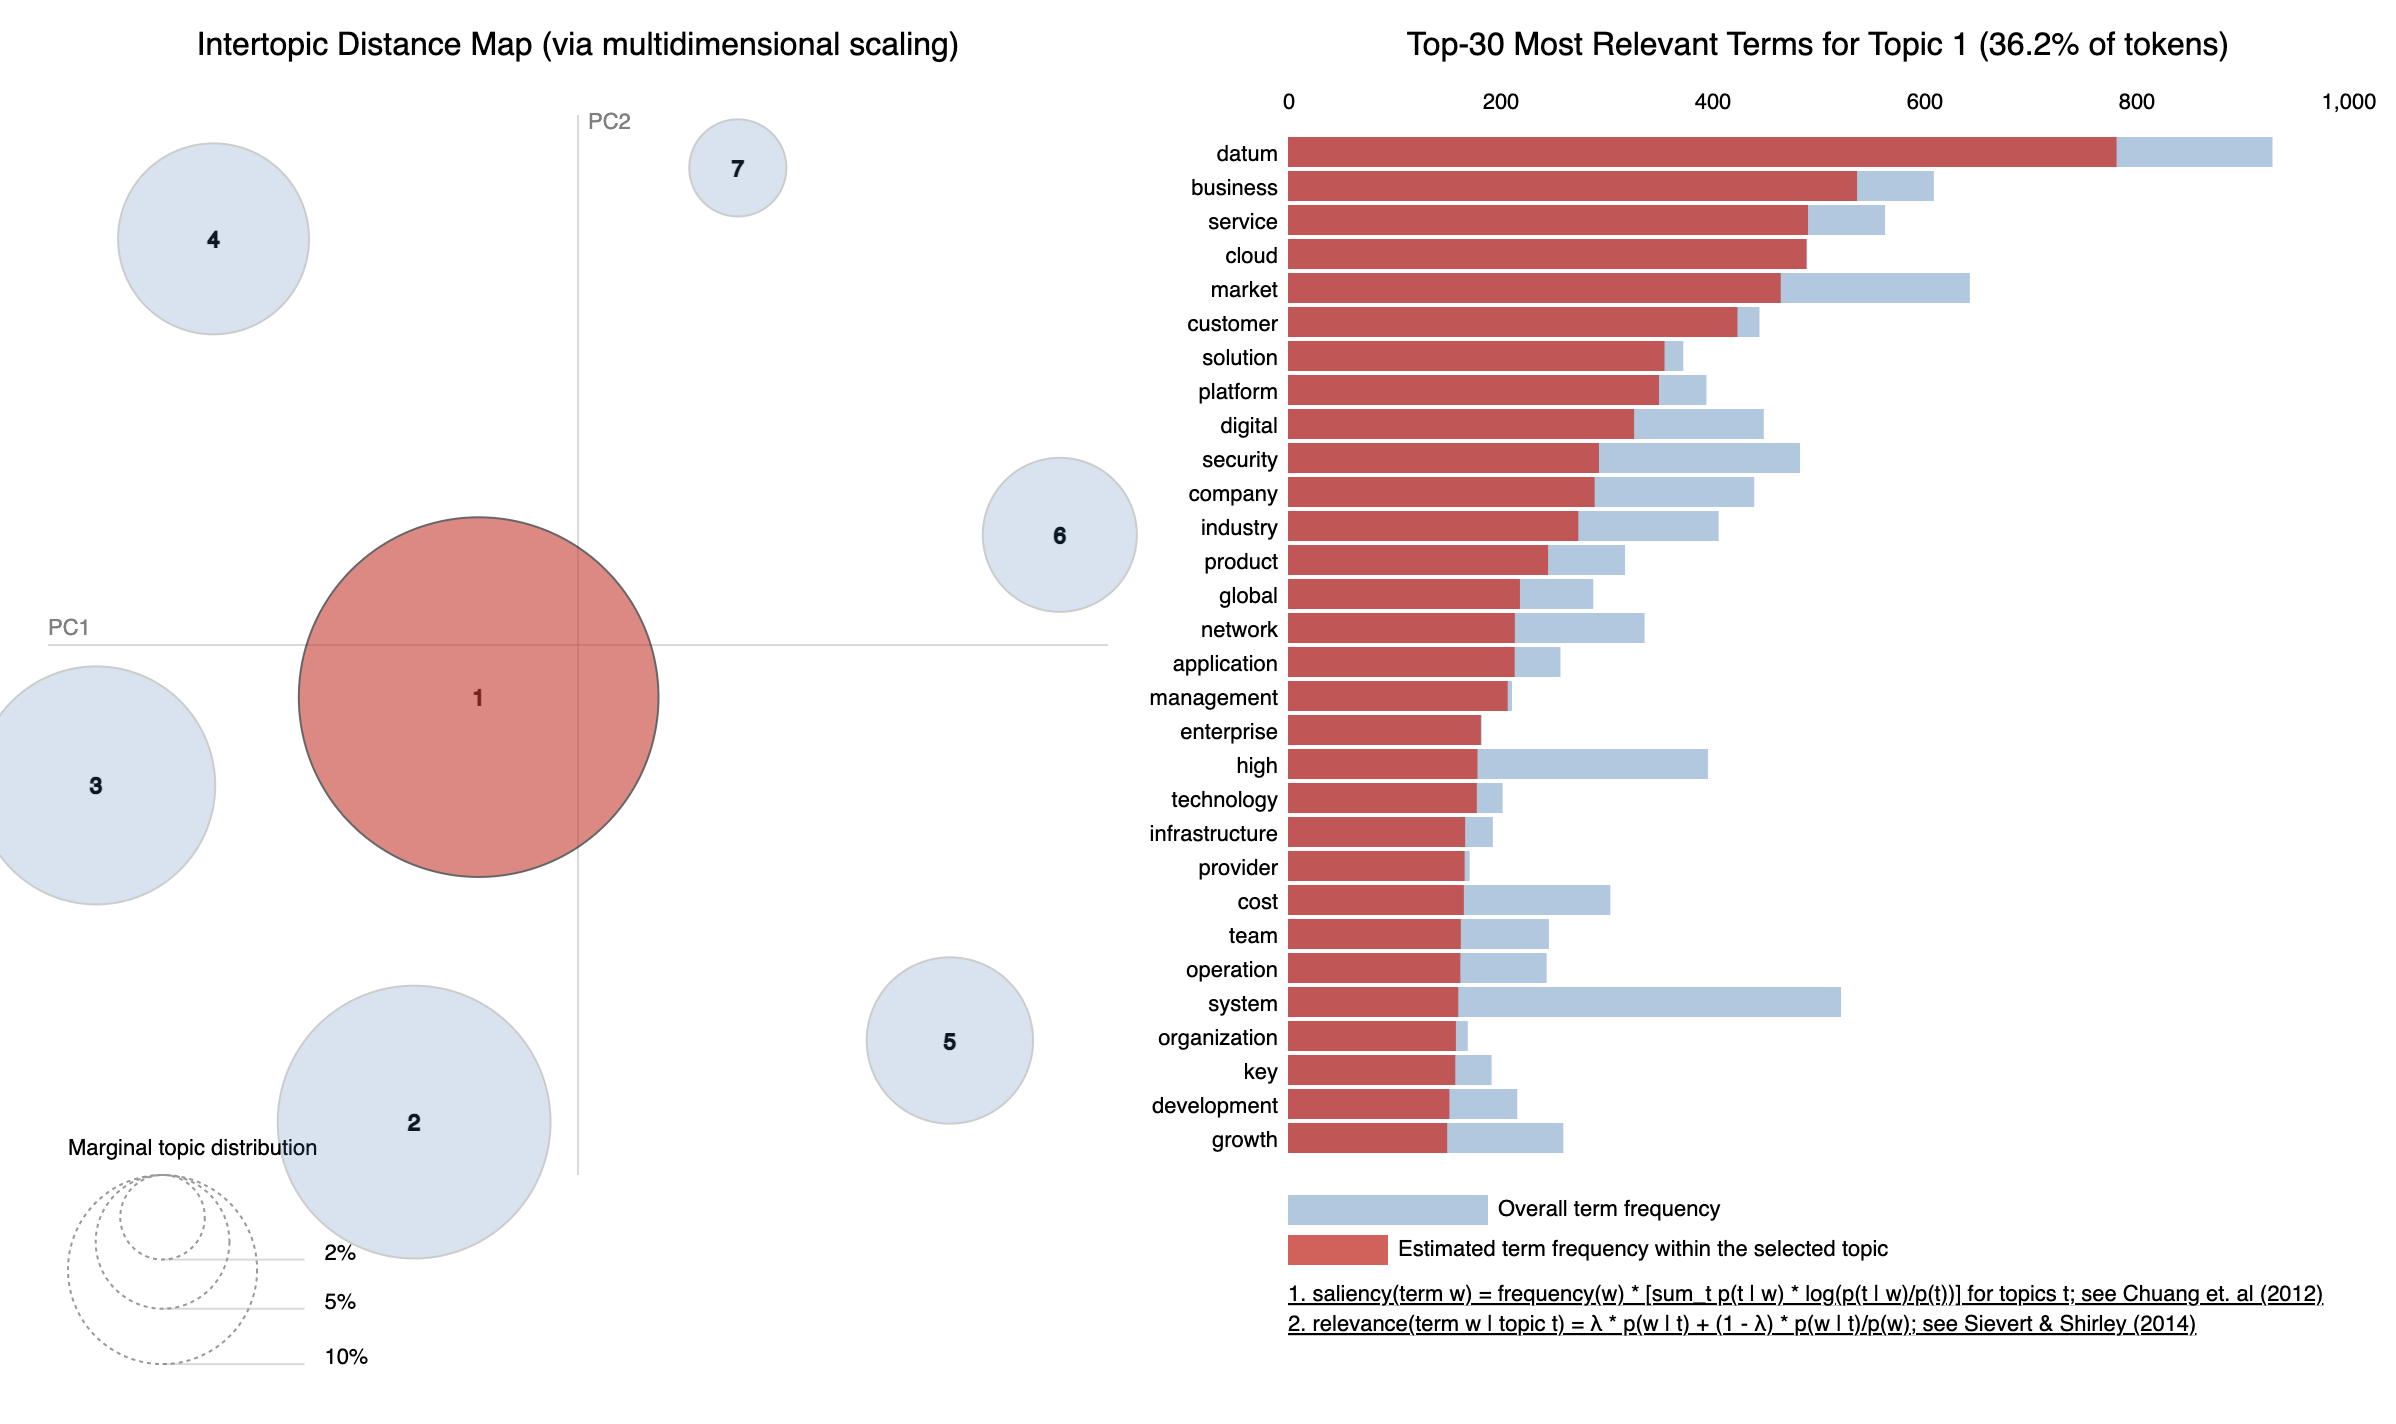
\includegraphics[width = 0.8\textwidth]{lda}
\end{center}             
        

            
            
            
            

            \quad The above shows the distribution of the topics with regards to percentage of tokens. From this figure and the previous, we can infer the most popular topic in the corpus in the selected timeframe.
            
\quad

\underline{Validation 1} 

            \quad Validation was performed by comparing the topic/ topics assigned, to the original keyword (category) used in querying the newsapi. Due to topics being constituted by multiple keywords, as long as the topic the article was assigned to contained the initial keyword, it was considered as correct. This was a logical step as it was unexpected for articles to have only a single category when articles cover multiple categories or topics to begin with. Using this approach we achieved a 89\% accuracy in the training set and a 83\% in the test set in predicting the original categories. Reducing the threshold for assigning topics to 0.15 resulted in an increased accuracy of 92.5\% and 90\% respectively but introduces more labels to the documents.

\quad

\underline{Validation 2}       
      
            \quad For the second validation, the top 5 articles from each topic assigned by the algorithm were used to determine whether the article was assigned to the correct topic(s). After reading through the article, one can assess if the topic it was assigned to was correct. As this part will be highly subjective we could set the threshold as the article having at least one correct topic. This means if the LDA topic we gave is "artificial intelligence" and after reading the sampled article and labelling it the same topic, we consider this to be labelled correctly. This was done for both the training set and the test set.
            

\begin{center}
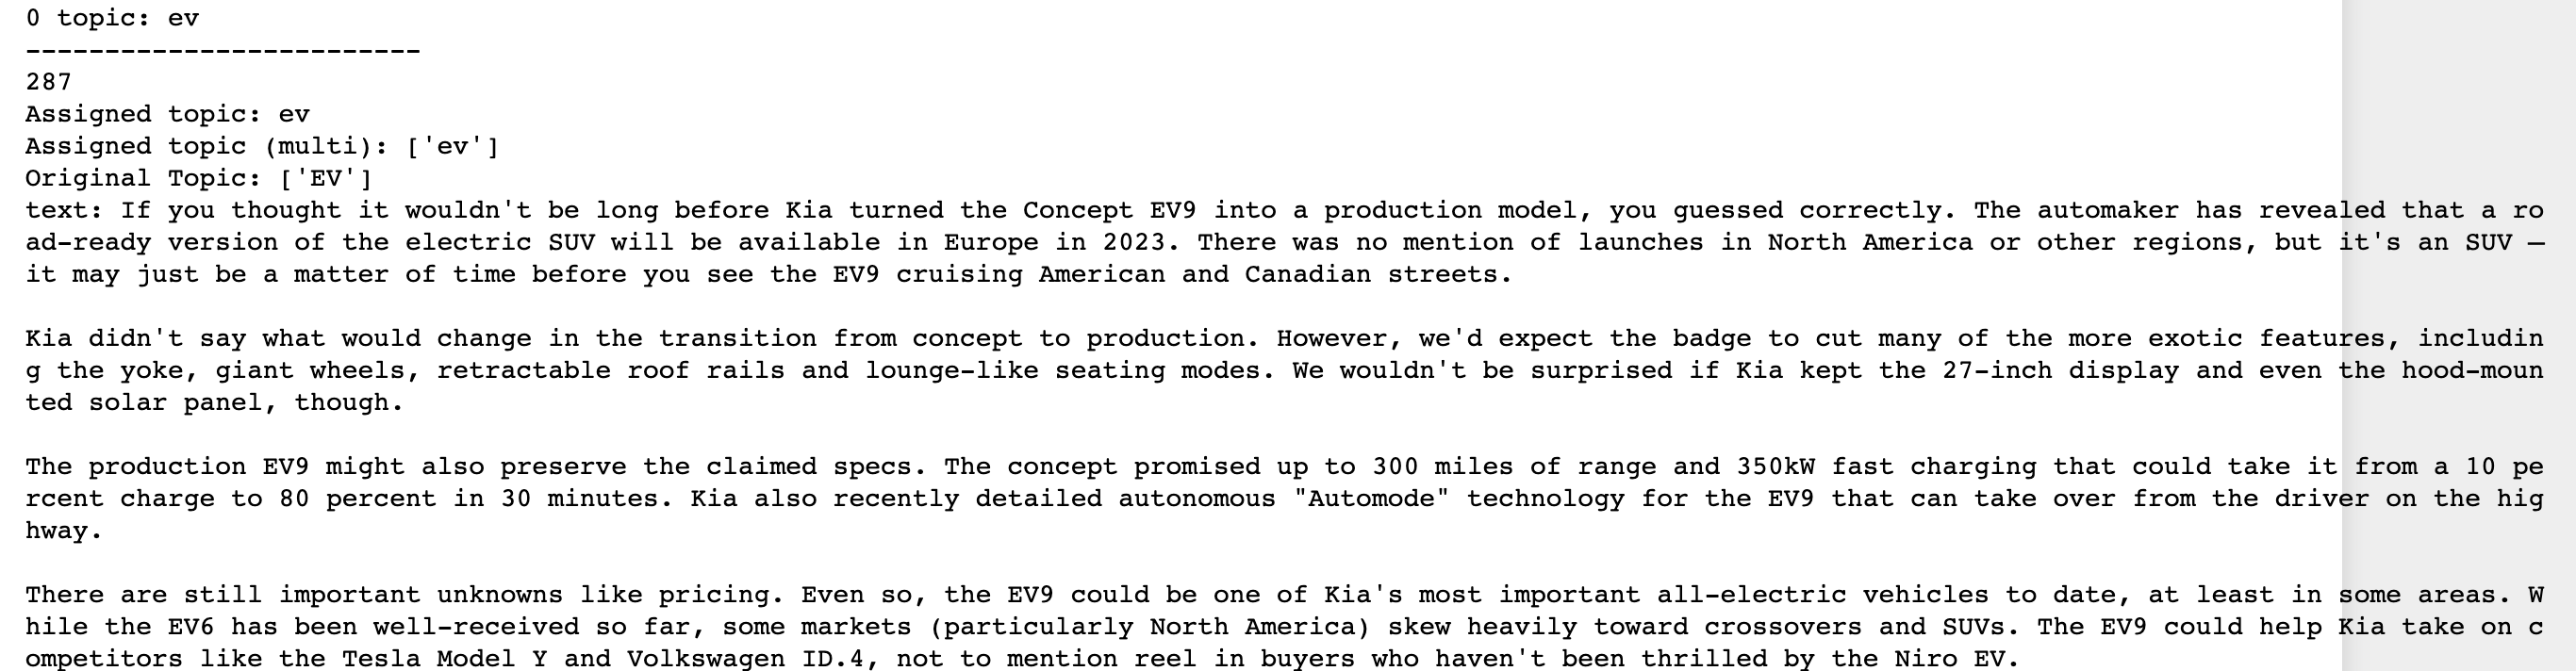
\includegraphics[width = 0.9\textwidth]{validation}
\end{center}            
            
            \quad From the above, it can be inferred that the topic of EVs is correct as the paragraph is referring to the Kia's model EV9 and mentions competitors such as Tesla. 


\begin{center}
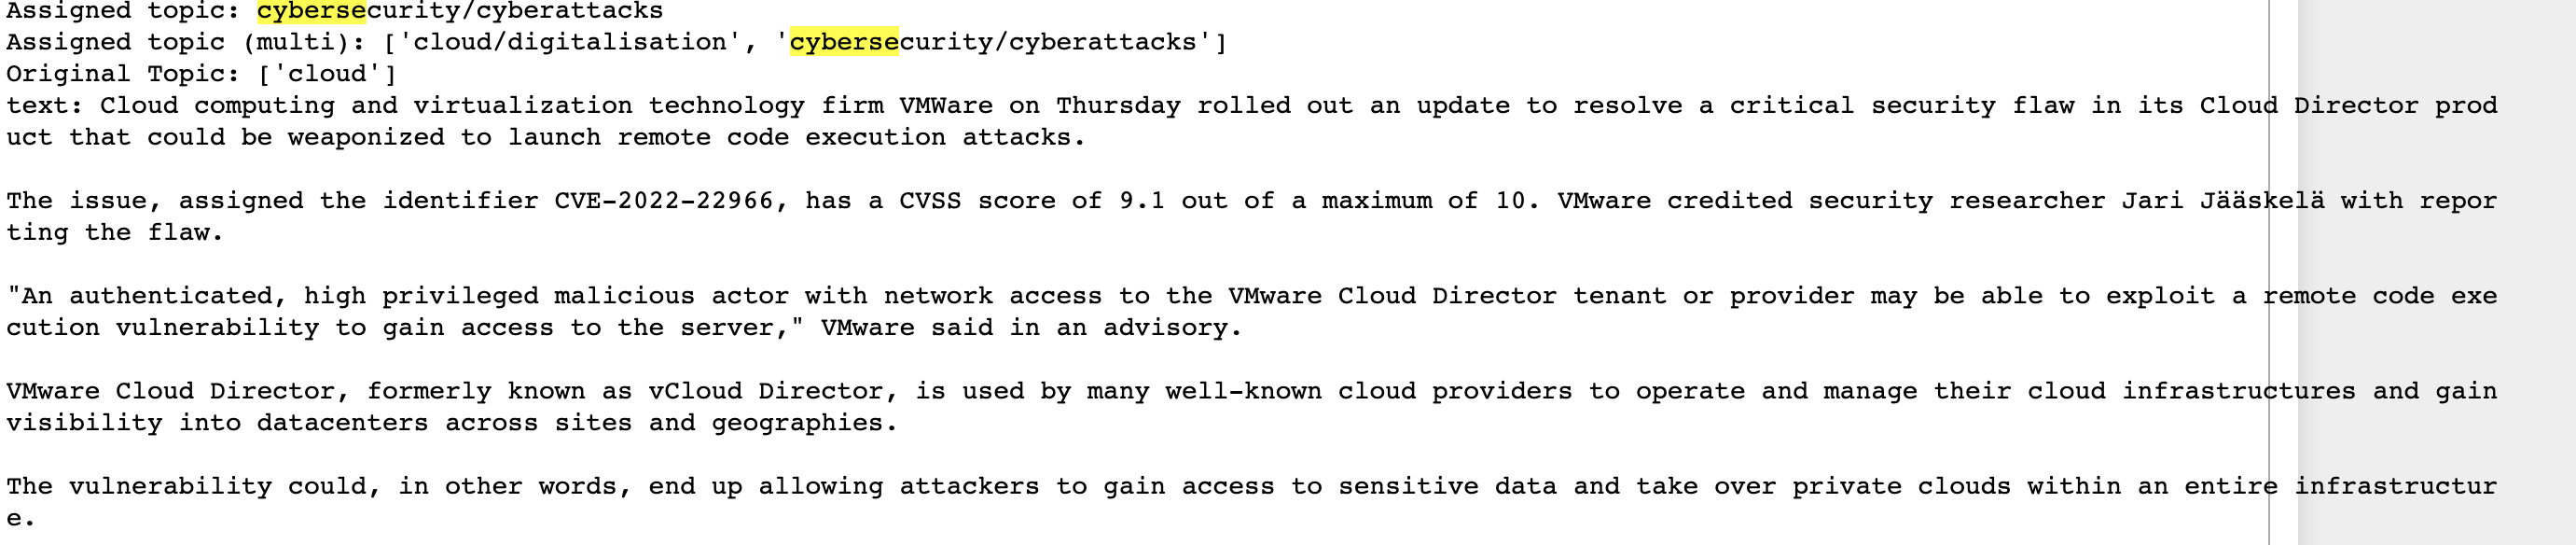
\includegraphics[width = 0.9\textwidth]{validation4}
\end{center}     
			\quad Another example would be this article which talks about cloud computing with respect to cybersecurity where VMware rolled out a patch to resolve a security flaw in its cloud product. Hence, after evaluation, we believe that the topic assigned to the article is appropriate and it explains more compared to its original topic of cloud computing.
            
\begin{center}
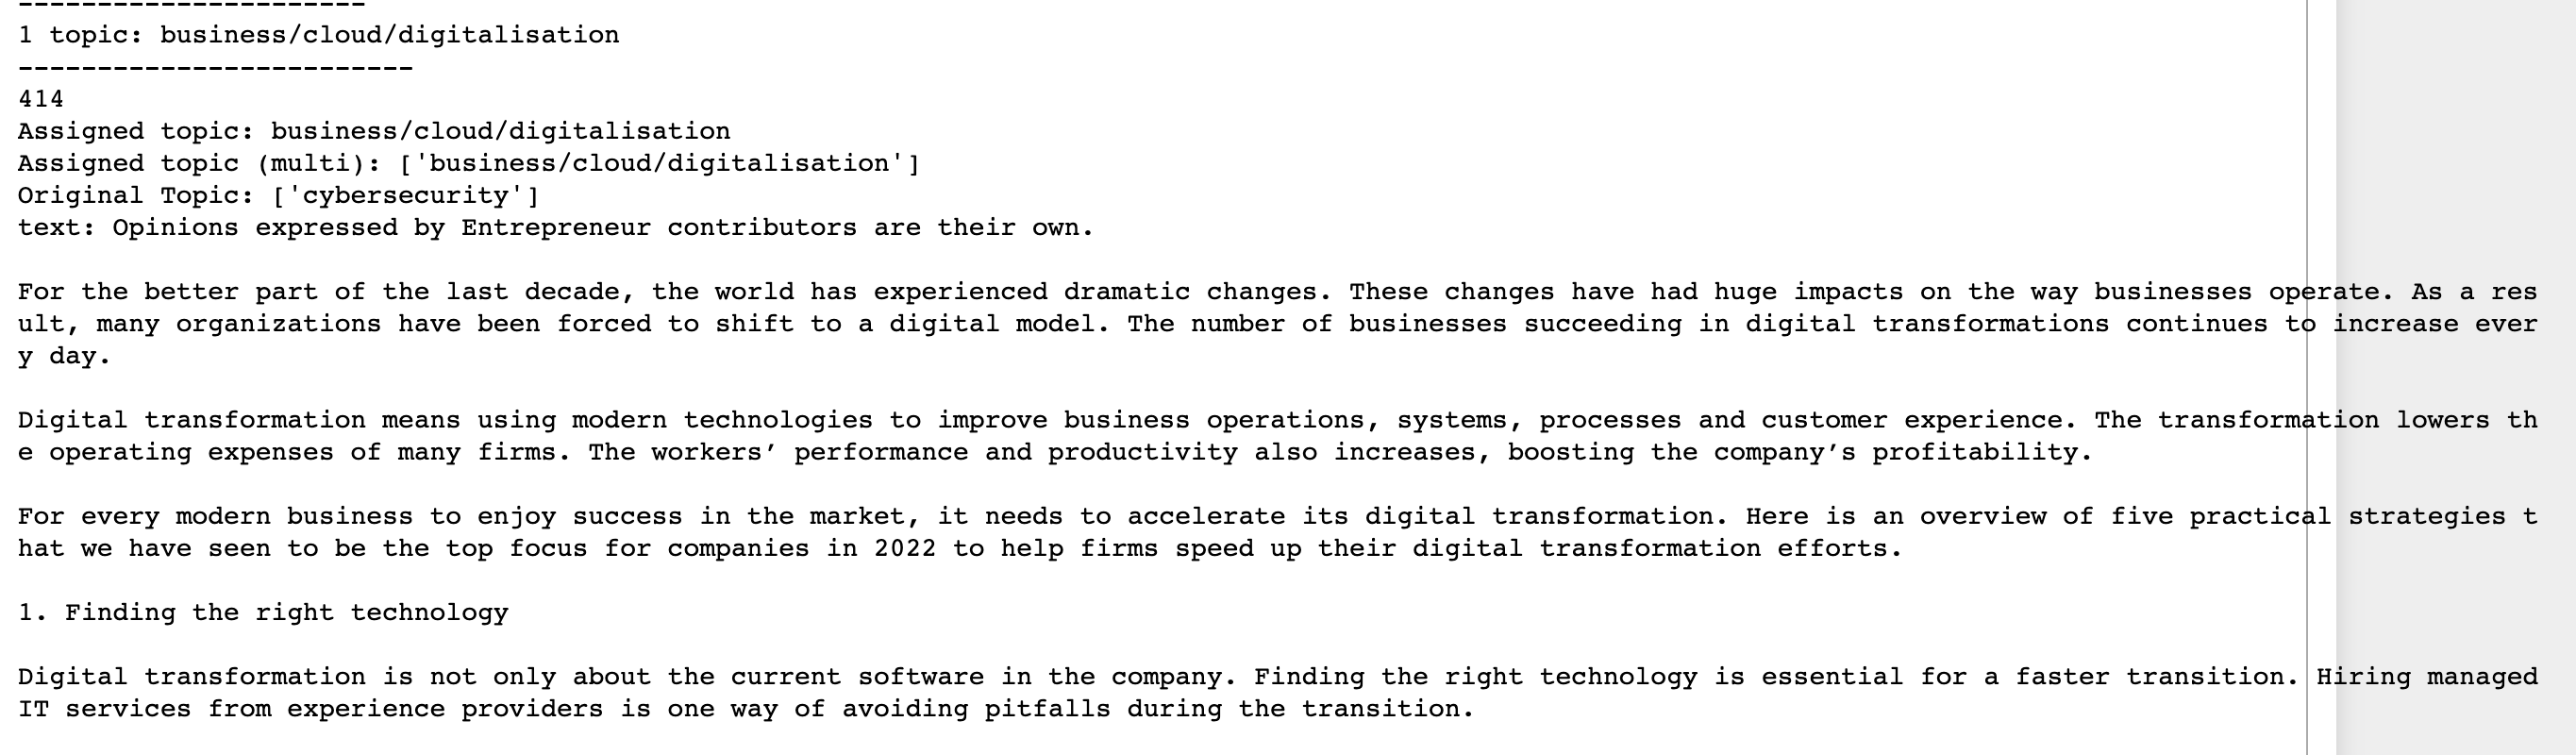
\includegraphics[width = 0.9\textwidth]{wronglabel}
\end{center} 
            \quad Using the second validation approach, most of the articles contained their originally assigned categories. For the above article, the algorithm correctly classified the article under business/cloud/digitalisation (which covers businesses,services) organizations while the original category of cybersecurity was not representative. The article explains methods to speed up digital transformation for businesses, whereas cybersecurity was mentioned as a sidenote in the article.
            
            \begin{center}
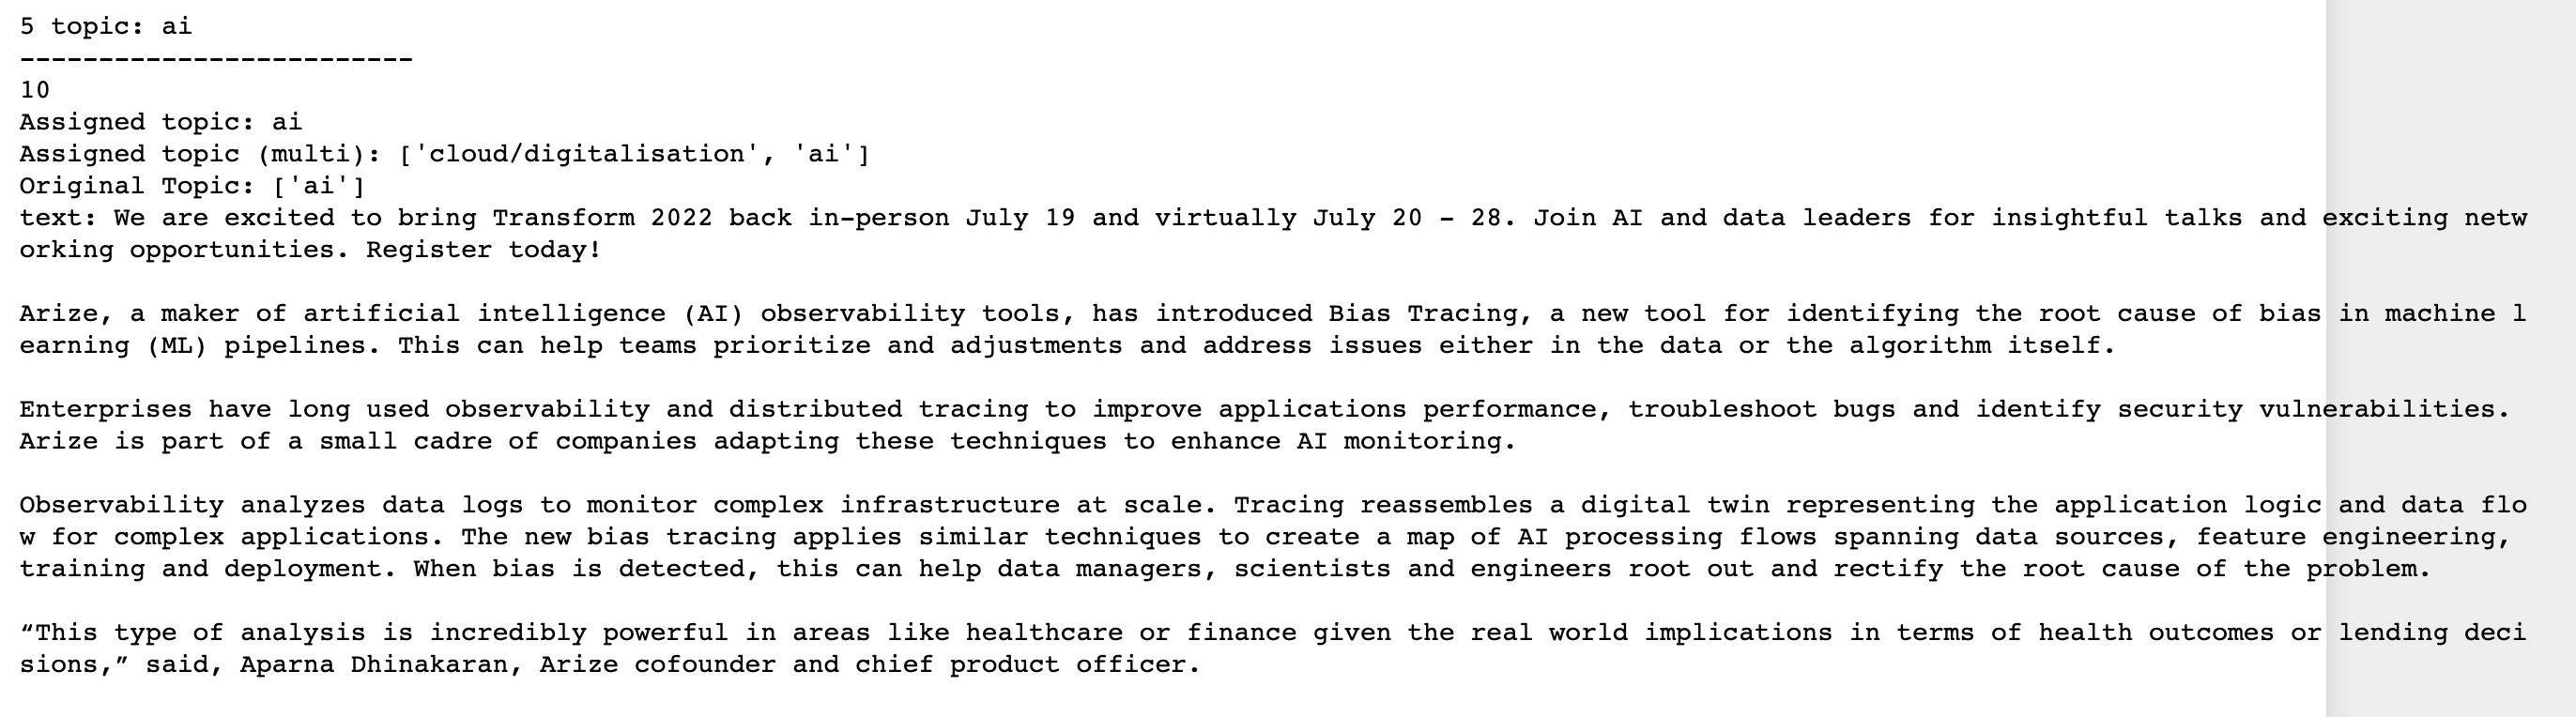
\includegraphics[width = 0.9\textwidth]{validation5}
\end{center} 

            \begin{center}
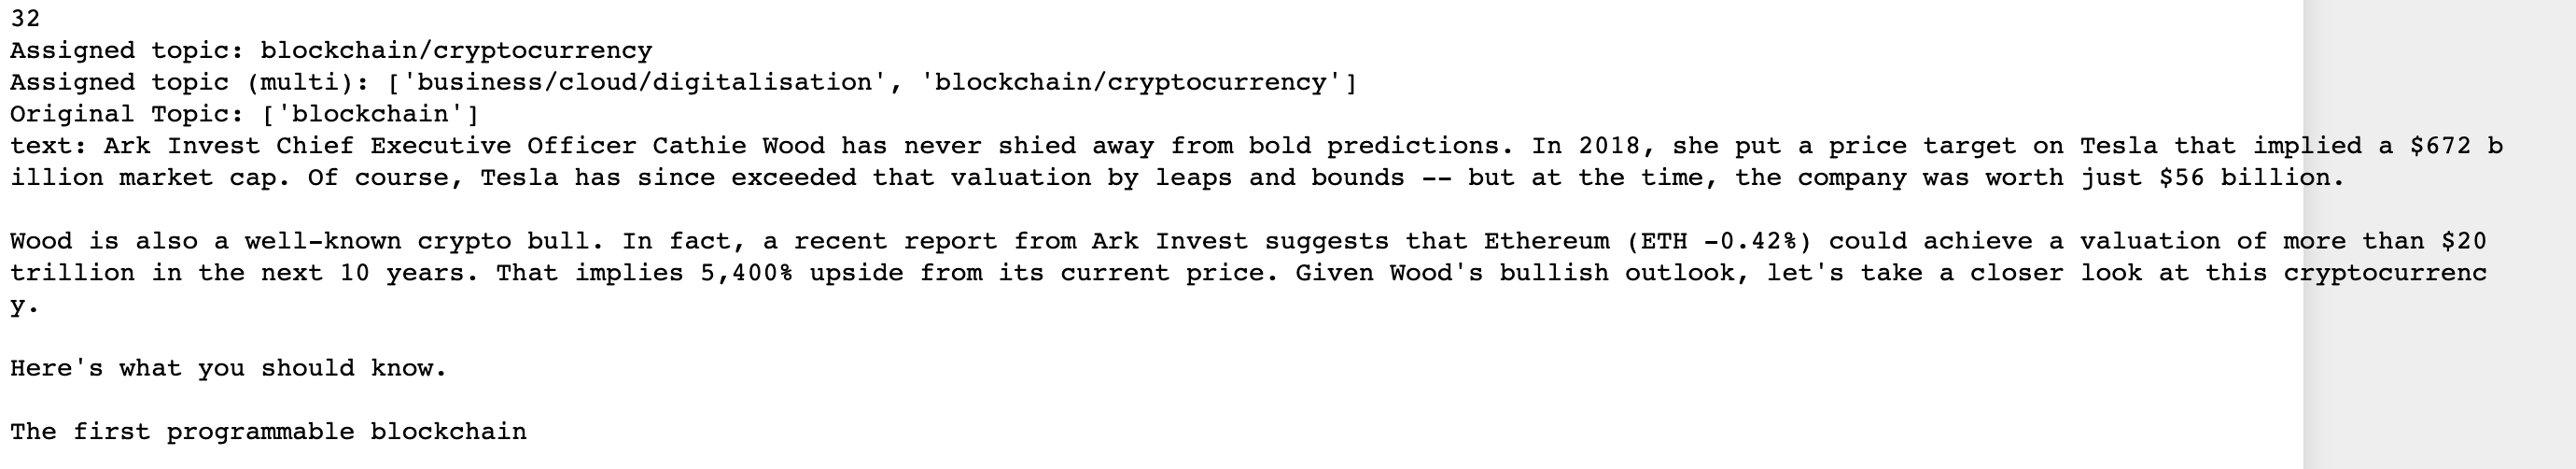
\includegraphics[width = 0.9\textwidth]{validation6}
\end{center} 
            
            \quad The same validation was done for the test set. We observe that the topic model was able to predict the correct topics for the test set as shown from the above examples.
            
                \begin{center}
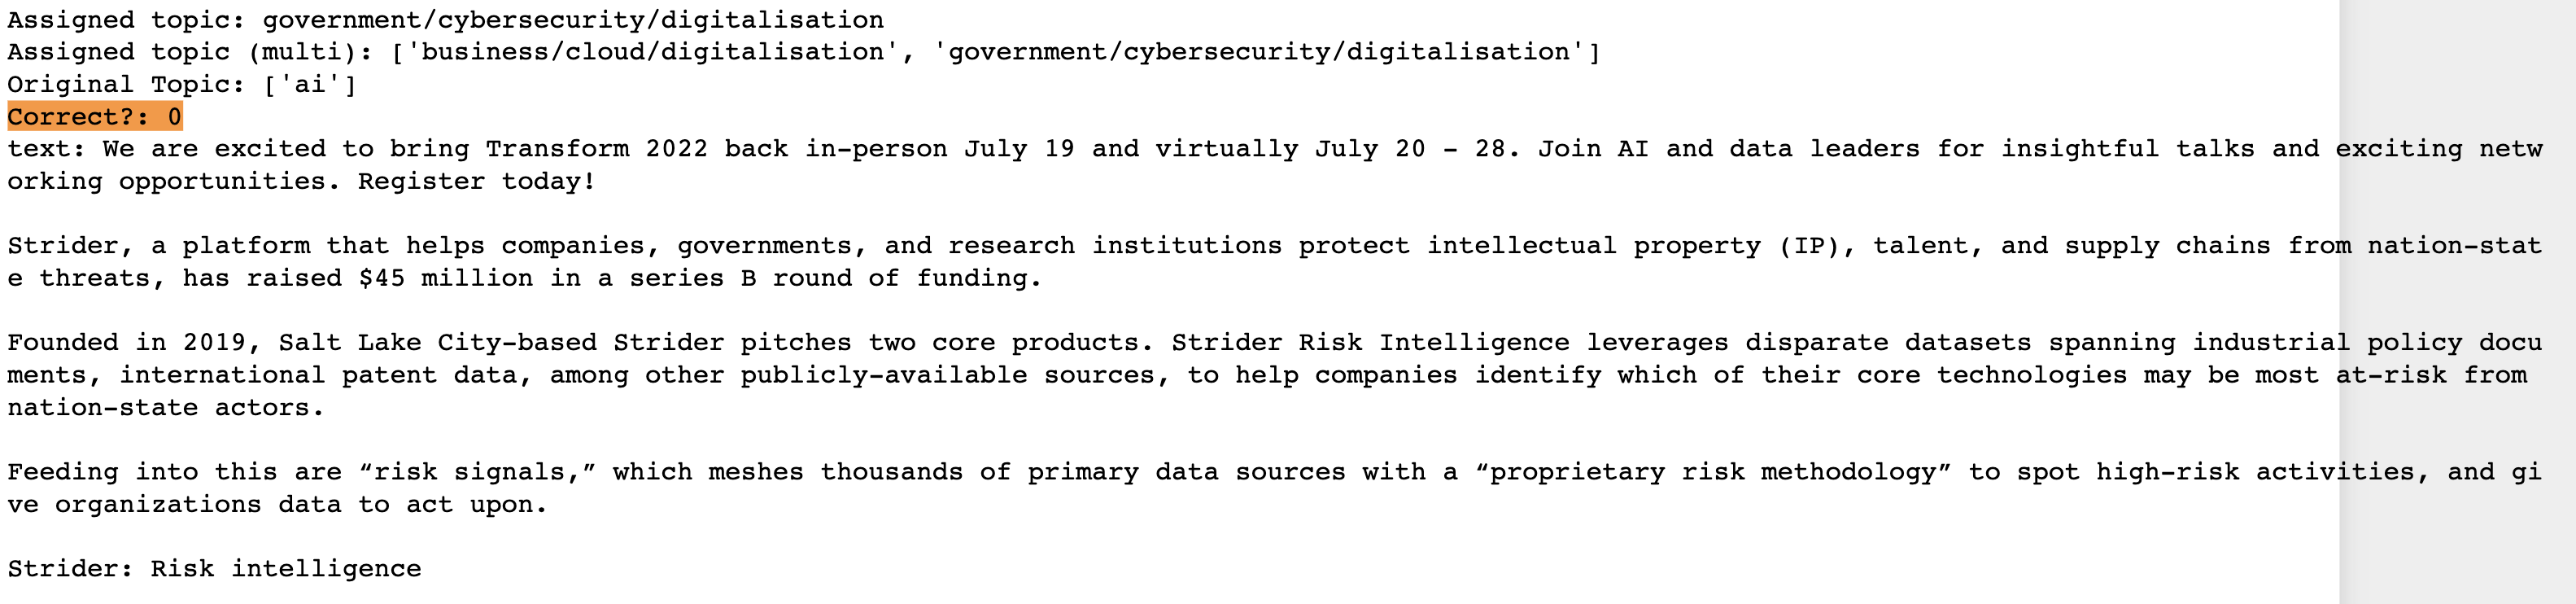
\includegraphics[width = 0.9\textwidth]{wrong}
\end{center} 

    \begin{center}
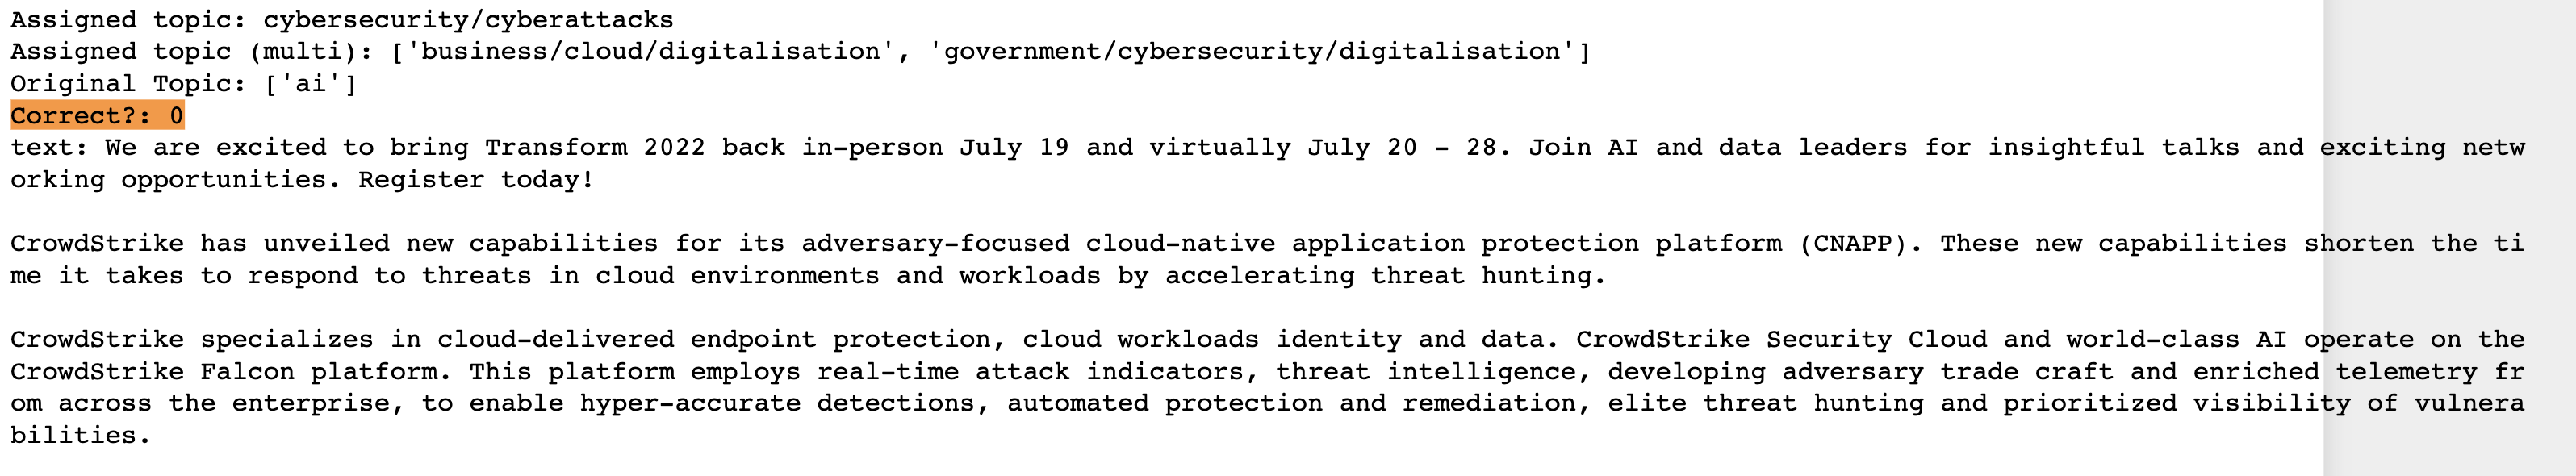
\includegraphics[width = 0.9\textwidth]{wrong2}
\end{center} 

			\quad However, there are instances where the model was not able to predict the original category of the article. This was because the article contained  more information related to the assigned topic (by the lda model) and only a few words containing the original category (such as ai).  The above articles demonstrate the following: the article is regarding a cloud application with cybersecurity capabilities, yet the original category was ai.
            
          \pagebreak
            
\underline{Validation 3}  
               
            \quad A good lda model would usually be interpretable (Roder et al., 2015) and a way to measure this is using coherence score. Coherence measures the similarity of words within a topic generated by the model. The more similar words are within a topic, the higher the coherence score and the better the model.
            \quad A way to measure coherence is based on Normalized Pointwise Mutual Information (NPMI).  Elements of vectors defined using NPMI were found to be highly correlated with human topic coherence ratings which are considered the gold standard (Roder et al., 2015). A context vector of word w takes the occurrence of 5 surrounding words (before and after) in relation to w forming a vector. This means that in a word vector, the jth element of $w_i$ will have the formula:
            $$NPMI(w_i,w_j)^\gamma   = ( \frac{log \frac{P(w_i,w_j) +\epsilon}{P(w_i)P(w_j)}}{-log(P(w_i,w_j) +\epsilon})^\gamma$$     

		\quad From the plot of the coherence score below,we observe that having 7 topics result in the highest coherence score of 0.53. As this score was the best, and the topics yielded were understandable, the finalised model contained 7 topics.
\begin{center}		
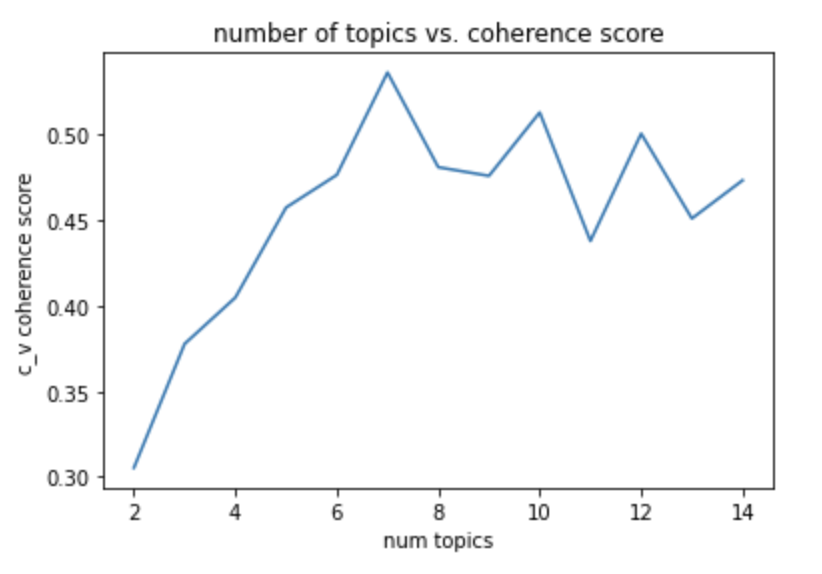
\includegraphics[width = 0.7\textwidth]{coherencescore}
\end{center}
 
\pagebreak

\underline{Validation 4}


		$$PP(W) = P(w_1,w_1...w_N)^{-\frac{1}{N}}=\sqrt[N]{\frac{1}{P(w_1,w_1...w_N)}}$$
		

		\quad The perplexity of the model is a metric which reflects how well a model will perform on a new set of data. According Jurafsky and Martin, the perplexity of a model on the test set is the inverse probability on the test set. It is known as an intrinsic measure for evaluating a natural language model. The higher the perplexity the better the model performs on unseen data. For this study we compared the perplexity of the training set to the test set. In gensim, the model outputs a log of perplexity causing the values to be negative. This means that a less negative perplexity will be better than a more negative one. The perplexity on the train set was -7.87 while the test set was -9.15. The difference is not too large and it is normal for a models. A plot of perplexity versus the number of topics (on the test set) shows that the bottom the curve is about 7 or 8  topics, this lends support to the current model.
		
	\begin{center}
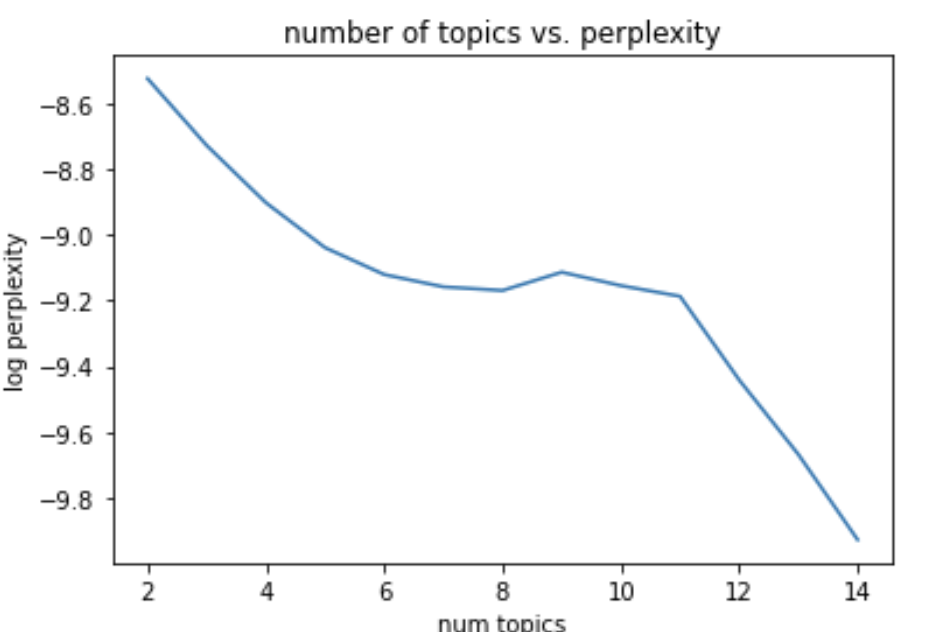
\includegraphics[width = 0.7\textwidth]{perplexity}

\end{center}
		 \pagebreak
		 
\underline{Results}
            
            \quad The results of this project is the assignment of these topics to articles. With this we can track the trending topics over a period of time. This could be in the form of a simple visualization (multi line charts with the count of topics on the y axis and date on the x axis. 
                 
\begin{center}
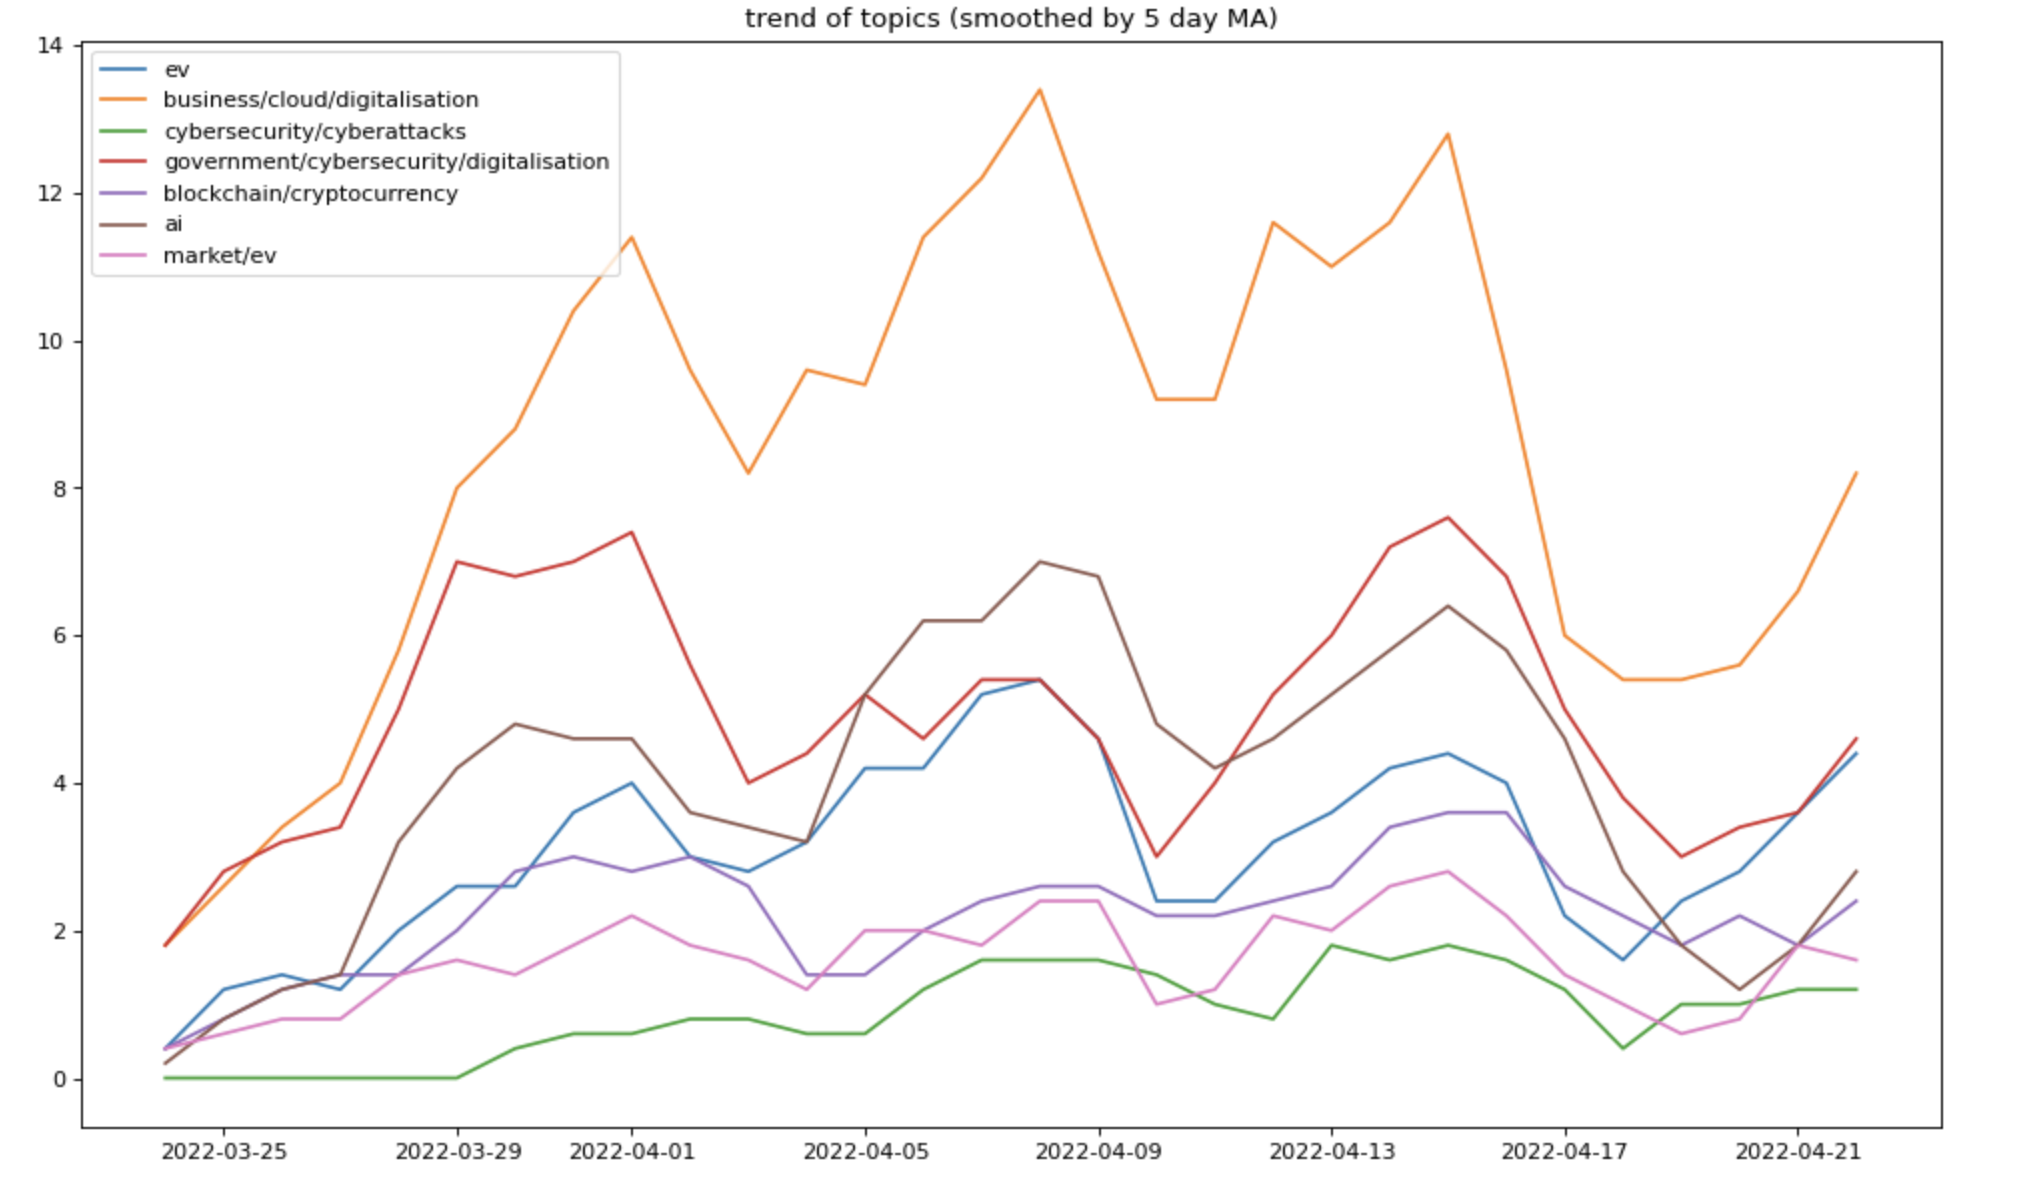
\includegraphics[width = 0.9\textwidth]{linecharts}

\end{center}
            
            \quad From the line chart of the topic 3 topics, we see that business/cloud/digitalisation is the most dominant topic and we can view a sharp spike from 2 Apr 2022. government/cybersecurity/digitalisation follows the trend of the former but has less of a spike. Moreover, while both topics started with the same number, the former became more popular over time as compared to the latter.
            
            \quad A second interesting point would be when a topic becomes more popular than another. For example, in the period of 5 Apr to 10 Apr, artificial intelligence superceded government/cybersecurity/digitalisation as the second hottest topic. Therefore, using this visualisation, a company could monitor technology trends and it could serve as a guide for their overall strategy. 
            
            
          \item[] \textbf{Potential Limitations}
          
          \quad A possible limitation of the approach would be that topics might shift over time and having a fixed number of topics could result in the model being unable to pick out newer topics. To counter this issue, the number of topics chosen has to be tweaked over time to account for different topics emerging.
          
          \quad Secondly, the queried keywords might not necessarily reflect the all the topics discussed within an article. Articles tend to be interdiscplinary and cover a range of topics. There have been instances where the topic model was able to pick up the topic better than the original categories. Therefore, the first validation method was limited by the accuracy of the original categories.
          
          \quad This leads to the next point that as LDA is an unclassified machine learning algorithm, the results might not fit neatly into the original categories. Take for example  the output of weighted tokens per topic, we see digitalisation present in multiple topics, instead of forming its own topic. Hence, the the second validation approach is required to ensure that the topics match the assigned categories. This in turn requires human intuition and effort to evaluate the articles and could be difficult to implement with datasets with more than 20 topics.
          
          \quad Lastly, as the number of articles is small, with only a months worth of data, the topic model is affected by topics which are recent. This issue can be solved by obtaining articles across a longer period to ensure that topics will be more stable across time. Additionally, most projects run topic models on a larger corpus of about 100,000 documents. Therefore, while this project has demonstrated satisfying results with a small corpus, a further improvement would be to collect more data and train the model on a larger corpus.
          
           \item[] \textbf{Conclusion}
          
          \quad This project aimed to find the most trending topics in technology over a time period and was able to demonstrate the ability to do so with the use of LDA. With the knowledge of these trends, organisations have a better understanding of the applications in different areas of tech and are better able to make decisions regarding long term strategies. As the dataset is limited in this study,  we believe that with a larger dataset, the topic model will yield more stable topics allowing organizations to keep better track of the shifting trends.
  \pagebreak  
  
        
\underline{References}

\quad Blei, D. M., Ng, A. Y., \& Jordan, M. I. (2003). Latent
Dirichlet allocation. Journal of Machine Learning Research, 3, 993–1022.

\quad Gan, J. \&  Qi, Y. (2021). Selection of the optimal number of topics for LDA Topic Model—taking patent policy analysis as an example. Entropy, 23(10), 1301. https://doi.org/10.3390/e23101301 

\quad Jurafsky , D. \& Martin J. H.,  (2021). Speech and Language Processing (pp. 8–9). Draft. 

\quad Röder, M., Both, A., \&; Hinneburg, A. (2015). Exploring the space of topic coherence measures. Proceedings of the Eighth ACM International Conference on Web Search and Data Mining. https://doi.org/10.1145/2684822.2685324 

        \end{itemize}
	
	\pagebreak

\end{titlepage}


\end{document}

